\documentclass[final]{beamer}
\mode<presentation>
{
  \usetheme{I6pd2ck}      %  you may also need to modify beamerthemeI6pd2ck.sty
}
\graphicspath{{figures/}} %  where you have your logos and figures

\def\red{\color{red}}

\usepackage{times}
\usepackage{amsmath,amssymb}
\usepackage[english]{babel}
\usepackage[latin1]{inputenc}
\usepackage{graphicx}



%%%%%%%%%%%%%%%%%%%%%%%%%%%%%%%%%%%%%%%%%%%%%%%%%%%%%%%%%%%%%%%%%%%%%%%%%%%%%%%%%%%%%%%%%%%%%%%%%%%
% MODIFY height and width appropriately.
% height and width are in cm
\usepackage[orientation=portrait,size=custom,height=80,width=111,scale=1.4,debug]{beamerposter} 

% Set \columnheight slight smaller than height above.
\newlength{\columnheight}
\setlength{\columnheight}{65cm}
%%%%%%%%%%%%%%%%%%%%%%%%%%%%%%%%%%%%%%%%%%%%%%%%%%%%%%%%%%%%%%%%%%%%%%%%%%%%%%%%%%%%%%%%%%%%%%%%%%%


\title{The very very very long poster title is placed here}
\author{Changhyun Kwon, First Name Last Name}
\institute{University of South Florida, Department of Industrial and Management Systems Engineering}
\date{\today}








\begin{document}


%%%%%%%%%%%%%%%%%%%%
\begin{frame}
\begin{columns}
%%%%%%%%%%%%%%%%%%%%








%%%%%%%%%%%%%%%%%%%%
\begin{column}{0.32\textwidth}
\begin{beamercolorbox}[center,wd=\textwidth]{postercolumn}
\begin{minipage}[T]{.95\textwidth}
\parbox[t][\columnheight]{\textwidth}{
%%%%%%%%%%%%%%%%%%%%


	\begin{block}{Hazardous Materials (hazmat)}
  	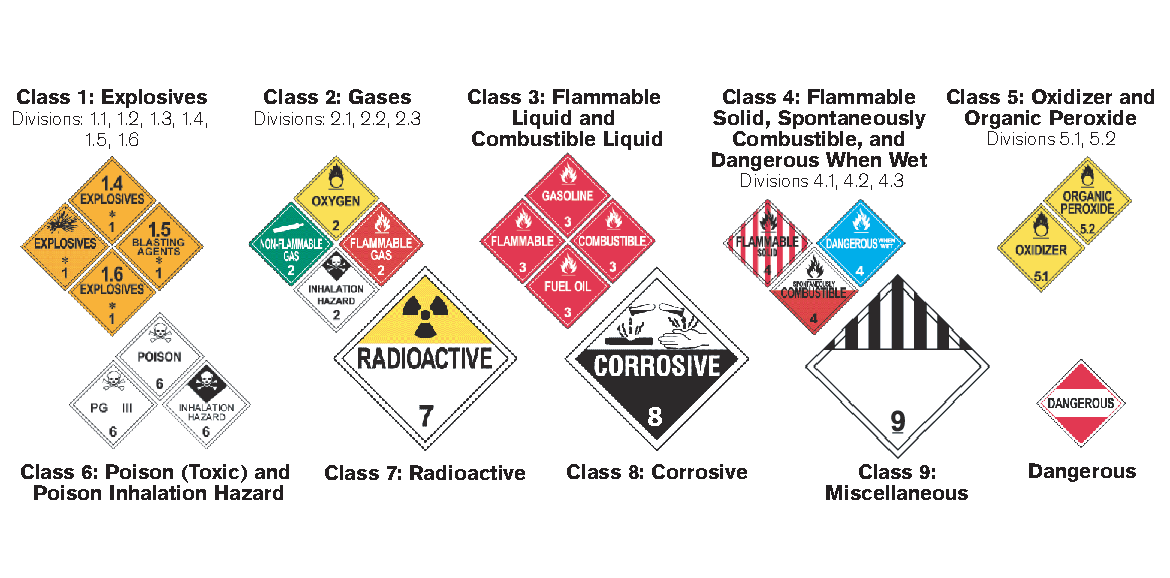
\includegraphics[width=0.9\textwidth]{yellowcard2}
	\end{block}

  \begin{block}{Number of hazmat incidents in 2000-2009 }
    \begin{table} \centering \small
    \begin{tabular}{|c|r|r|}
    \hline Mode & No. of Incidents & Percentage \\ 
    \hline Air & 13,232 & 7.89 \\ 
    \hline Highway & 146,120 & 87.09 \\ 
    \hline Rail & 7,987 & 4.76 \\ 
    \hline Water & 446 & 0.27 \\ 
    \hline Total & 167,785 & 100 \\ 
    \hline 
    \end{tabular} 
    \end{table}
  \end{block}

  \begin{block}{How to Control Network Flows?}
    \begin{itemize}
    \item Network Design Approach
    	\begin{itemize}
    	\item Close/Open road segments
    	\item Increase capacity of road segments
    	\end{itemize}
    \item Toll System Approach
    	\begin{itemize}
    	\item Charge tolls to vehicles traveling certain road segments
    	\end{itemize}
    \end{itemize}
  \end{block}


  \begin{block}{Block Title Here}
  	\begin{itemize}
  	\item abcdefg
  	\item abcdefg
  	\item abcdefg
  	\item abcdefg
  	\item abcdefg
  	\end{itemize}
  \end{block}
  


%%%%%%%%%%%%%%%%%%%%
}
\end{minipage}
\end{beamercolorbox}
\end{column}
%%%%%%%%%%%%%%%%%%%%
%%%%%%%%%%%%%%%%%%%%
\begin{column}{0.32\textwidth}
\begin{beamercolorbox}[center,wd=\textwidth]{postercolumn}
\begin{minipage}[T]{.95\textwidth}
\parbox[t][\columnheight]{\textwidth}{
%%%%%%%%%%%%%%%%%%%%


  \begin{block}{Risk Measure and Travel Delay}
    \begin{itemize}
    \item We consider a \emph{\red duration-population-frequency} risk measure:
    \[
    R_a(v_a,u_a) = s_a(v_a) \rho_a u_a
    \]
    where $\rho_a$ is the population exposure along the arc.
    \item The linear travel delay function is:
    \[
    s_a(v_a) = t_a \left( 1 + v_a / C_a \right)
    \]
    \end{itemize}
  \end{block}



  \begin{block}{Case Study for Albany, NY (46 nodes and 70 arcs)}
    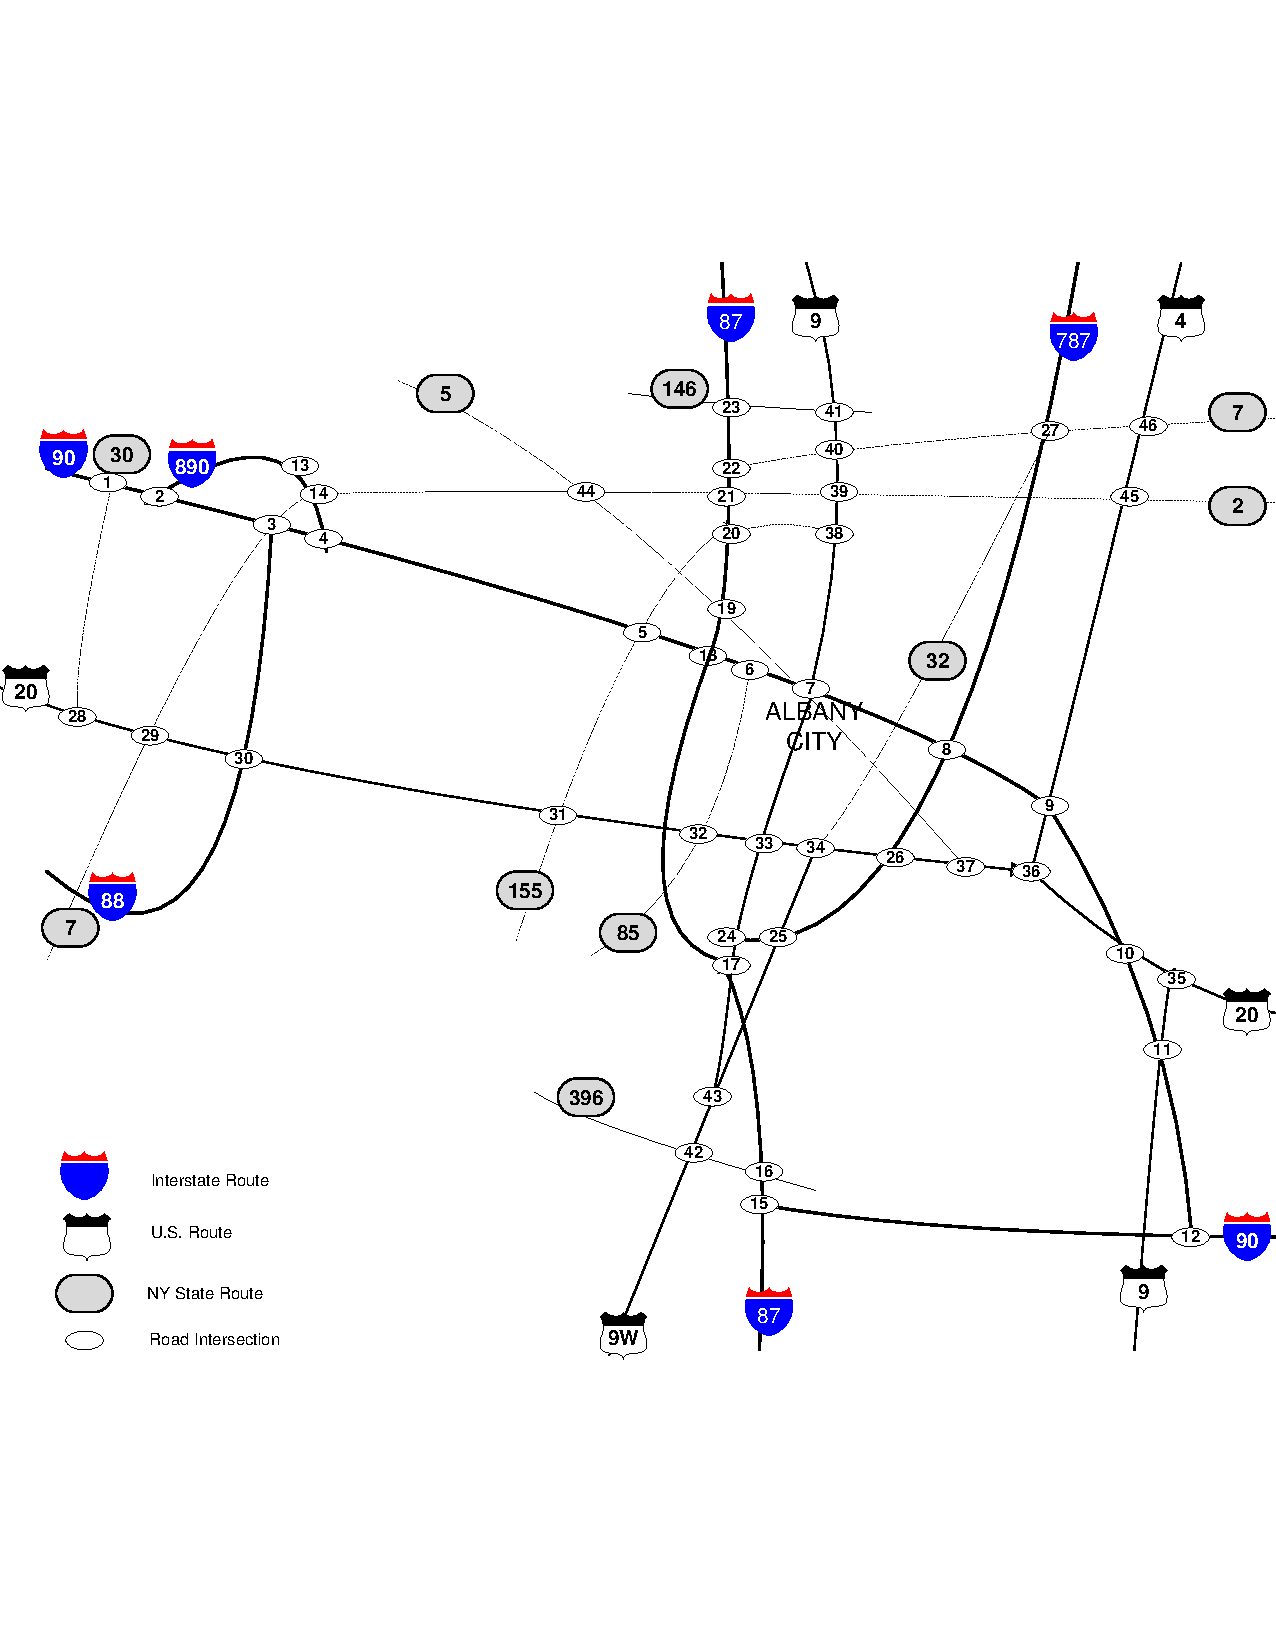
\includegraphics[width=0.7\textwidth]{map_albany}
  \end{block}


  \begin{block}{Block Title Here}
  	\begin{itemize}
  	\item abcdefg
  	\item abcdefg
  	\item abcdefg
  	\item abcdefg
  	\item abcdefg
  	\end{itemize}
  \end{block}
  
  \begin{block}{Block Title Here}
  	\begin{itemize}
  	\item abcdefg
  	\item abcdefg
  	\item abcdefg
  	\item abcdefg
  	\item abcdefg
  	\end{itemize}
  \end{block}



%%%%%%%%%%%%%%%%%%%%
}
\end{minipage}
\end{beamercolorbox}
\end{column}
%%%%%%%%%%%%%%%%%%%%
%%%%%%%%%%%%%%%%%%%%
\begin{column}{0.32\textwidth}
\begin{beamercolorbox}[center,wd=\textwidth]{postercolumn}
\begin{minipage}[T]{.95\textwidth}
\parbox[t][\columnheight]{\textwidth}{
%%%%%%%%%%%%%%%%%%%%


  \begin{block}{Results}
    \begin{table} \centering \footnotesize
    \begin{tabular}{|c|c|c|c|c|c|}
    \hline
    $(w_1,w_2,w_3)$ & Risk & Delay (regular) & Delay (hazmat) & Toll (regular) & Toll (hazmat)\\ \hline
    $(10^{-4},1,1)$ & $-15.09 \%$ & $3.95 \% $ & $-0.27\% $ & $1.29 \times 10^9 $ & $1.66 \times 10^3$\\
    \hline
    $(10^{-3},1,1)$ & $-22.07 \%$ & $4.68 \% $ & $-1.39\% $ & $1.31 \times 10^9$ & $1.66 \times 10^3$\\
    \hline
    $(1,1,1)$ & $-24.70\%$ & $22.61\% $ & $-39.61\% $ & $5.29 \times 10^6$ & $0$\\ \hline
    $(10^2,1,1)$ & $-24.70 \%$ & $25.99 \% $ & $-39.52\% $ &$0$  & $0$\\
    \hline $(10^5,1,1)$ & $-24.70 \%$ & $25.99 \% $ & $-39.52\% $ & $0$
    & $0$
    \\
    \hline
    \end{tabular}
    \caption{Results with various $w_1$ with given $w_2 = 1$ and $w_3 =1$}
    \label{tbl:result1} 
    \end{table}
    
    \begin{table} \centering
    \footnotesize
    \begin{tabular}{|c|c|c|c|c|c|}
    \hline
    $(w_1,w_2,w_3)$ & Risk & Delay (regular) & Delay (hazmat) & Toll (regular) & Toll (hazmat)\\ \hline
    $(1,1,1)$ & $-24.70\%$ & $22.61\% $ & $-39.61\% $ & $5.29 \times 10^6$ & $0$\\ \hline
    $(1,10^5,1)$ & $-5.23\%$ & $2.86 \% $ & $4.89\% $ & $2.87 \times 10^8$ & $0$\\
    \hline
    $(1,10^8,1)$ & $-4.41 \%$ & $2.81 \% $ & $5.58\% $ & $2.62 \times 10^8$ & $0$\\
    \hline
    $(1,10^{12},1)$ & $-4.41 \%$ & $2.81 \% $ & $5.58\% $ & $2.62 \times 10^8$ & $0$\\
    \hline
    \end{tabular}
    \caption{Results with various $w_2$ with given $w_1 = 1$ and $w_3 =1$} 
    \label{tbl:result2} 
    \end{table}
    
    \begin{table} \centering
    \footnotesize
    \begin{tabular}{|c|c|c|c|c|c|}
    \hline
    $(w_1,w_2,w_3)$ & Risk & Delay (regular) & Delay (hazmat) & Toll (regular) & Toll (hazmat)\\ \hline
    $(10^{-4},1,10^5)$ & $-22.52 \%$ & $3.06 \% $ & $-11.9\% $ & $3.30 \times 10^7$ & 0\\
    \hline
    \end{tabular}
    \caption{Results with $(w_1, w_2,w_3)=(10^{-4}, 1 , 10^4)$}
    \label{tbl:result3}
    \end{table}
  
  \end{block}
  
  
  
  \begin{block}{Block Title Here}
  	\begin{itemize}
  	\item abcdefg
  	\item abcdefg
  	\item abcdefg
  	\item abcdefg
  	\item abcdefg
  	\end{itemize}
  \end{block}
  
  
  \begin{block}{Block Title Here}
  	\begin{itemize}
  	\item abcdefg
  	\item abcdefg
  	\item abcdefg
  	\item abcdefg
  	\item abcdefg
  	\end{itemize}
  \end{block}
  
  
  
  \begin{block}{Block Title Here}
  	\begin{itemize}
  	\item abcdefg
  	\item abcdefg
  	\item abcdefg
  	\item abcdefg
  	\item abcdefg
  	\end{itemize}
  \end{block}






%%%%%%%%%%%%%%%%%%%%
}
\end{minipage}
\end{beamercolorbox}
\end{column}
%%%%%%%%%%%%%%%%%%%%




%%%%%%%%%%%%%%%%%%%%
\end{columns}
\end{frame}
%%%%%%%%%%%%%%%%%%%%



\end{document}


%%%%%%%%%%%%%%%%%%%%%%%%%%%%%%%%%%%%%%%%%%%%%%%%%%%%%%%%%%%%%%%%%%%%%%%%%%%%%%%%%%%%%%%%%%%%%%%%%%%%
%%% Local Variables: 
%%% mode: latex
%%% TeX-PDF-mode: t